% !TEX root = TEX/writeup.tex/writeup.tex
\documentclass{article}
\usepackage{amsmath,amsfonts,graphicx,lipsum,geometry,caption,courier,listings,xcolor}
\author{Micah Gruenwald}
\title{Final Coding Write-Up: The Mandelbrot Set}
\date{December 2024}

\lstset{
tabsize = 4, %% set tab space width
showstringspaces = false, %% prevent space marking in strings, string is defined as the text that is generally printed directly to the console
numbers = left, %% display line numbers on the left
commentstyle = \color{green}, %% set comment color
keywordstyle = \color{blue}, %% set keyword color
stringstyle = \color{red}, %% set string color
rulecolor = \color{black}, %% set frame color to avoid being affected by text color
basicstyle = \small \ttfamily , %% set listing font and size
breaklines = true, %% enable line breaking
numberstyle = \tiny,
}
\begin{document}
\maketitle
\pagebreak
\section{Introduction : What is the Mandelbrot Set}
\begin{minipage}[t]{0.4\textwidth}
    You may be asking, what is the Mandelbrot set. Well, its a set of complex numbers. A complex is a number expressed as $a+bi$, and lies on a two dimensional plane, the complex plane, where cordinates are determined by $(a,b)$\\
    The Mandelbrot set is in turn the set of complex numbers z=($a+bi$), such that $\lim_{n\to\infty} z^n \neq  \infty$. This is hard to physically conceptualize, but in essense we are asking, if I indefinetly multiply this complex number by itself, will it get really big or will it stay small?
\subsection{How is it Rendered?}
We obviously cannot raise each and every number to the $\infty$, so our code chooses an iteration count, and raises each complex value to that count. It determines if the number diverges by checking is $\sqrt{a^2+b^2}>2$, becuase all complex numbers with that property do diverge. If we determine our value diverges, the loop breaks. The function returns the amount of iterations went through divided by the total itterations to show how close the number is to being in the mandelbrot set. This value says that it is rapidly divergent if we only get a value around $0$ and is in the Mandelbrot srt if we get $1$. Everything else is in that range. Each point in our image is colored in based on that value. 
\end{minipage}
\hspace{20pt}
\begin{minipage}[t]{0.4\textwidth}
    \captionof{figure}{Complex Plane Example}
    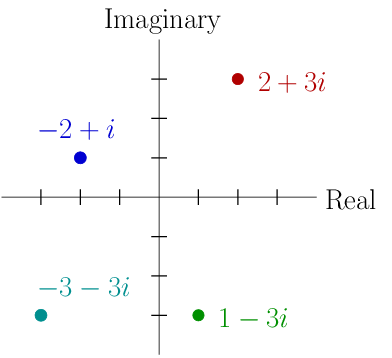
\includegraphics[width = \linewidth]{/Users/Period2/Desktop/VSCode/Mandelbrot-py/TEX/writeup.tex/Complex Plane.png}
    \textit{Image courtesy of galileospendulum.org}

    \vspace{20pt}
    \captionof{figure}{Mandelbrot Set Example}
    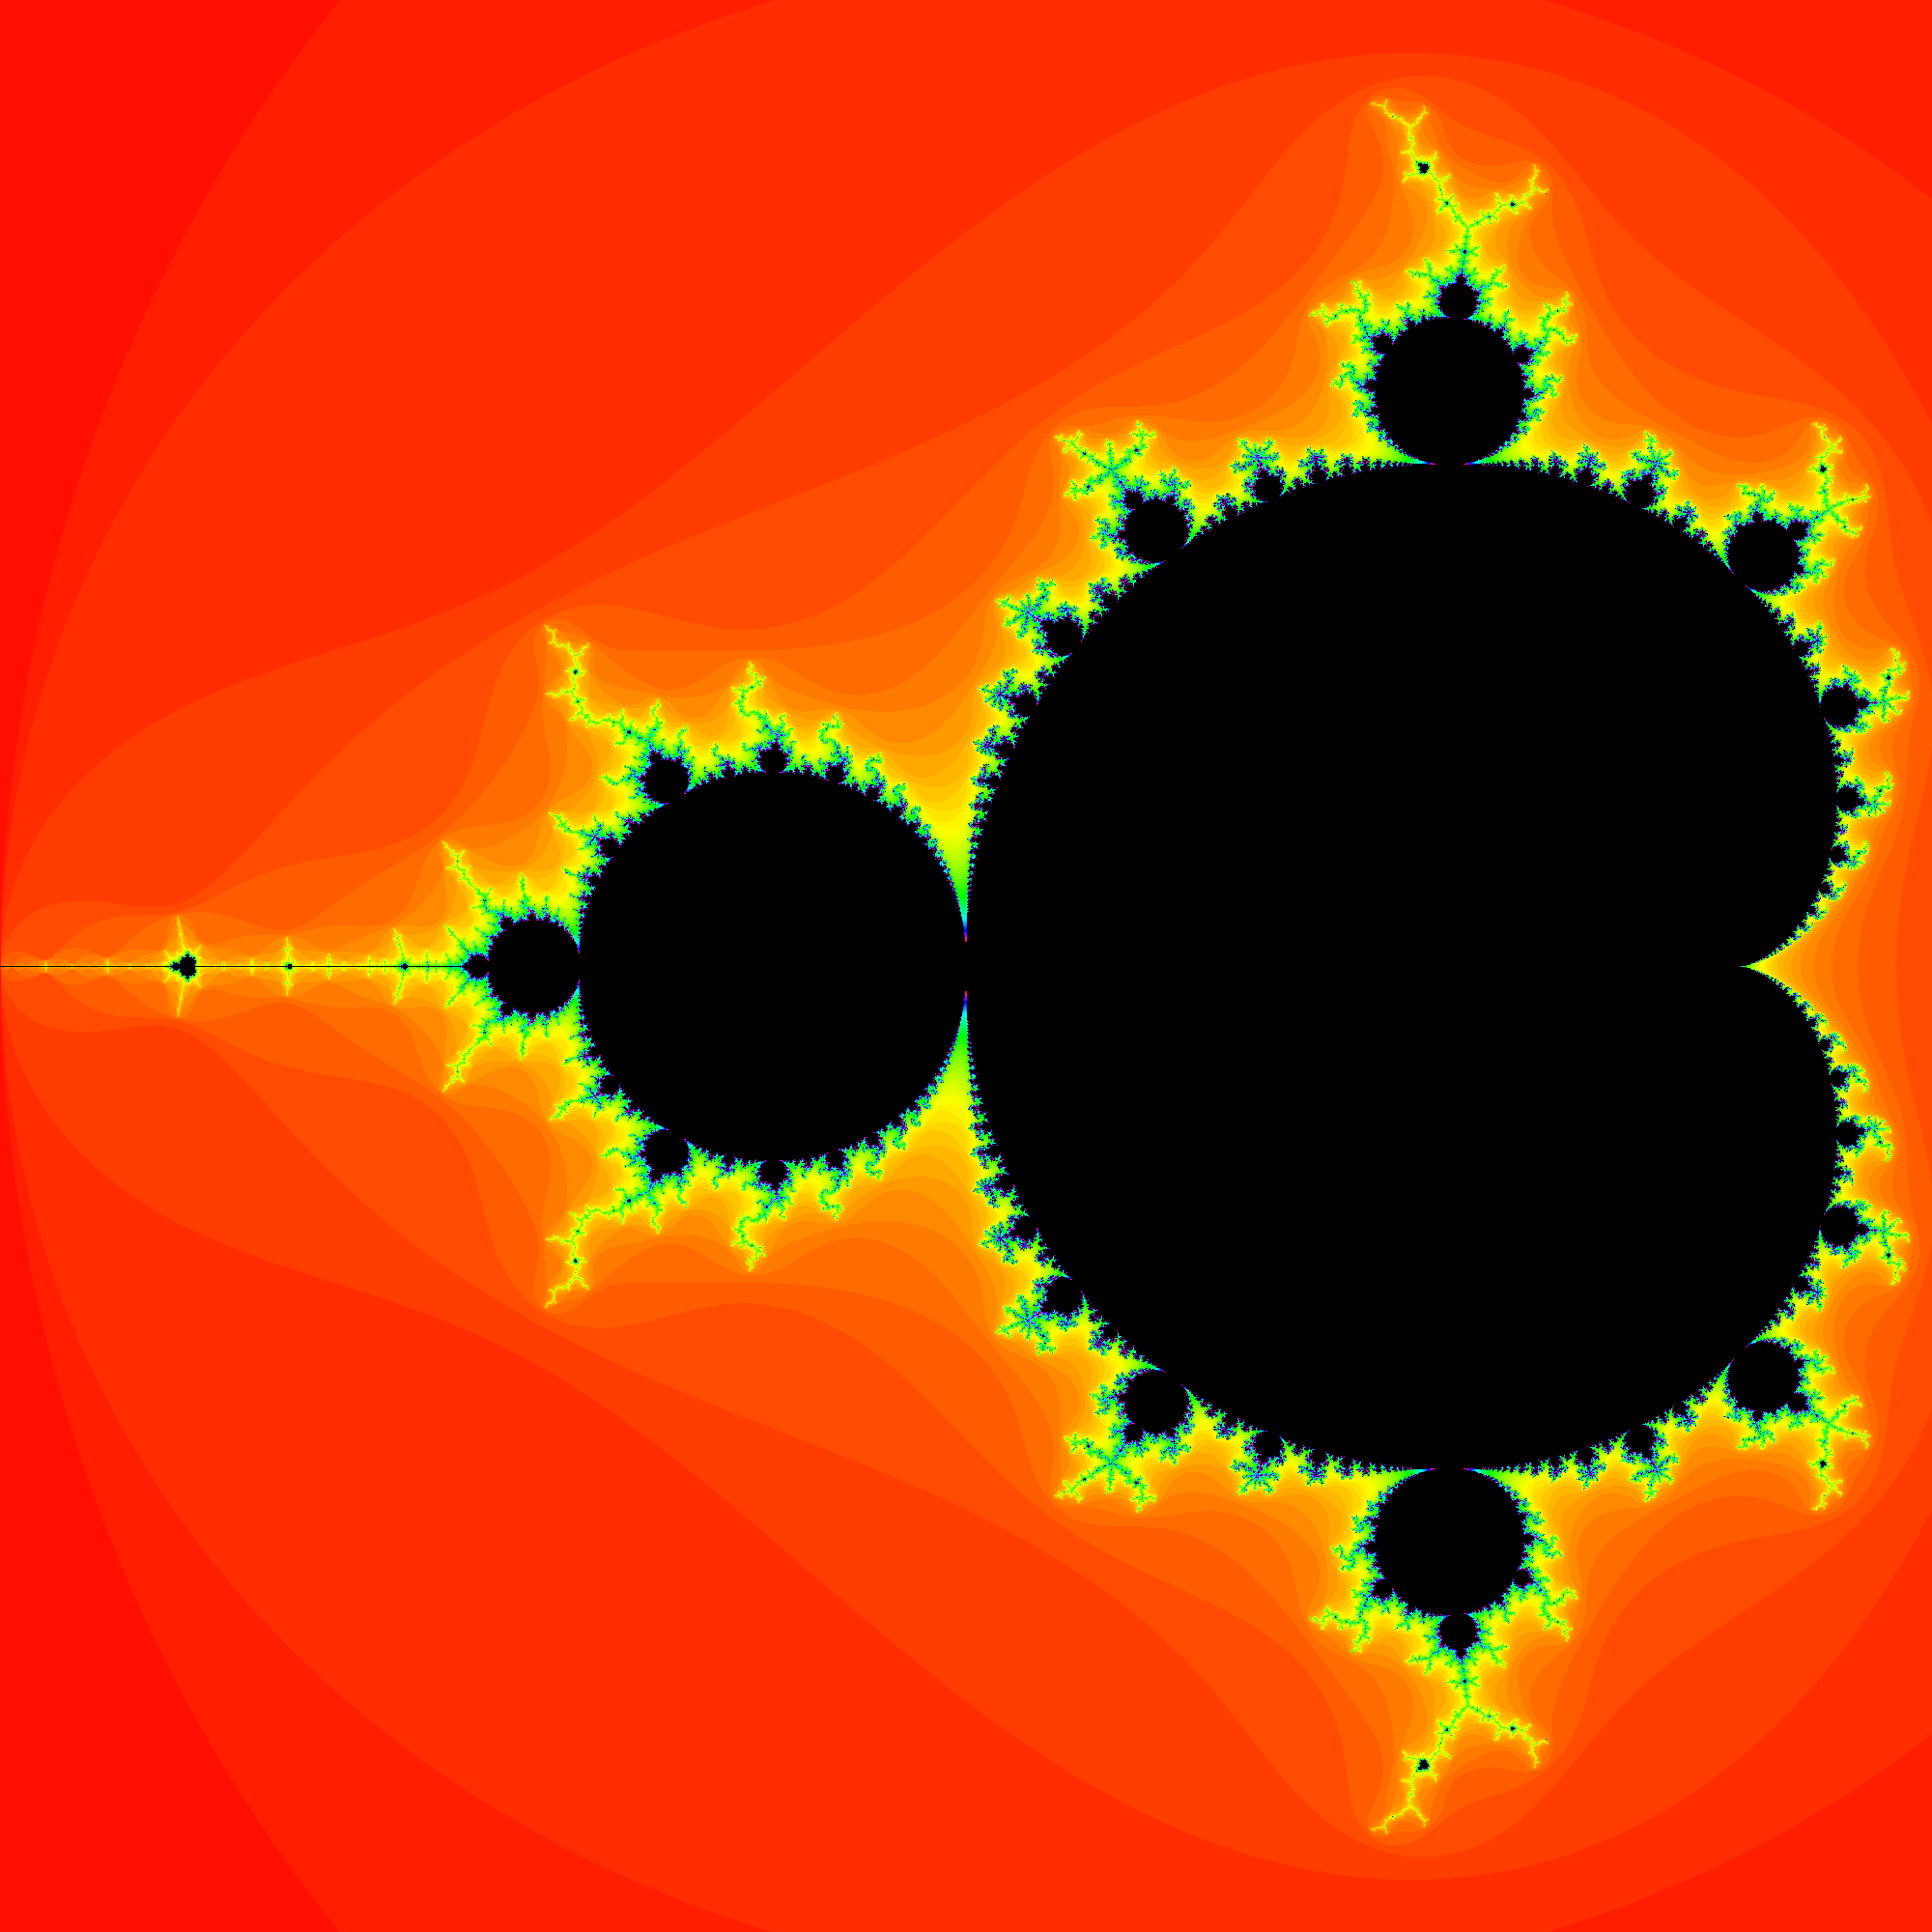
\includegraphics[width = \linewidth]{/Users/Period2/Desktop/VSCode/Mandelbrot-py/Saved Renders/Main Set.png}
\end{minipage}
\pagebreak
\section{Functions}
The code has a few basic fucntions: 
\begin{itemize}
    \item mandelbrotValue:
        This takes in the pixel coordiante of a spot in our image, and returns the mandelbrot value, between 0 and 1.
    \item pixelToPoint:
        This takes in a pixel in our image, and returns it's mapped coordinate on the complex plane. 
    \item color:
        This takes in a mandelbrotValue and returns a rgb color
    \item renderMandelbrot:
        This lists through the pixels of our image, and sets the color of each pixel to the color of the mandelbrotValue at that pixel. Finally, it writes an image file called render.png. 
\end{itemize}
\section{How the Code Works}
\begin{minipage}[t]{0.45\textwidth}
    \subsection{mandelbrotValue}
    We start by defining the function, taking in a point px and py.
    We then define variables. This code is a bit optimized but in essense the cordinate is the complex $x+yi$, and becuase compelx numbers multiply as they do, we can find our next value with the forumlae in the code. The function loops through the set, counting up iterations, and breaks when it finds the number diverges, finally returning a max iteration.
\end{minipage}
\hspace{20pt}
\begin{minipage}[t]{0.5\textwidth}
    \begin{lstlisting}[language = Python , frame = trBL , firstnumber = last , escapeinside={(*@}{@*)}]
def mandlebrotValue(px,py):
    point = pixelToPoint(px,py)
    x2 = 0
    y2 = 0
    w = 0
    iteration = 0
    while(x2+y2 <= 4 and iteration<maxIterations):
        x = x2 - y2 + point[0]
        y = w -x2 - y2 + point[1]
        x2 = x*x
        y2=y*y
        w = (x+y)*(x+y)
        iteration += 1
    return iteration/maxIterations
    \end{lstlisting}
\end{minipage}

\pagebreak
\begin{minipage}[t]{0.45\textwidth}
    \subsection{pixelToPoint}
    This is analagous to taking in\\ $\begin{bmatrix} \text{px}\\\text{py}\\1 \end{bmatrix}$\\ and returning\\ $\begin{bmatrix} \frac{\text{domainLength}}{\text{width}}& 0&\text{startX}\\ 0& \frac{\text{rangeLength}}{\text{height}}&\text{startY}\\0&0&1\end{bmatrix} \begin{bmatrix} \text{px}\\\text{py}\\1 \end{bmatrix}$
    \subsection{color}
    Takes in the madnelbrot lightness value. If it is 1 it returns black, otherwise it converts the lightness to a angle on the color wheel, and retruns the color at max saturation and brightness. 
    \subsection{renderMandelbrot}
    Lists through all of the pixels and assigns the tuple color value to each point as an elemnt fo a 2d array. Then it mpas that array onto an 8 int hex value, and finally it assigns that array to a png file. 
\end{minipage}
\hspace{20pt}
\begin{minipage}[t]{0.5\textwidth}
    \begin{lstlisting}[language = Python , frame = trBL , firstnumber = last , escapeinside={(*@}{@*)}]
def pixelToPoint(px,py):
    point=[500,500]
    point[0]= startX + px/width*domainLength
    point[1]= startY+ py/height*rangeLength
    return point
    \end{lstlisting}
\vspace{35pt}
    \begin{lstlisting}[language = Python , frame = trBL , firstnumber = last , escapeinside={(*@}{@*)}]
def color(lightness)
    if(lightness ==1):
      return (0,0,0)
    return tuple([255*x for x in hsv_to_rgb(lightness+indent,1,1)])
    \end{lstlisting}
\vspace{30pt}
\begin{lstlisting}[language = Python , frame = trBL , firstnumber = last , escapeinside={(*@}{@*)}]
def renderMandelbrot(output):
   pixels = [[color(mandlebrotValue(px,py)) for px in range(width)] for py in range(height)]
   array = np.array(pixels, dtype=np.uint8)
   img = Image.fromarray(array)

   img.save("/Users/Period2/Desktop/VSCode/Mandelbrot-py/movie/"+output+".png","JPEG")
            \end{lstlisting}
\end{minipage}
\pagebreak
\section{Renders}
\begin{minipage}[t]{0.45\textwidth}
    \captionof{figure}{Inside}
    
\includegraphics[width = \linewidth]{/Users/Period2/Desktop/VSCode/Mandelbrot-py/Saved Renders/Inside.png}
    \captionof{figure}{Sun Bay}
    
\includegraphics[width = \linewidth]{/Users/Period2/Desktop/VSCode/Mandelbrot-py/Saved Renders/Sun bay.png}
    \captionof{figure}{Micahbrot}
    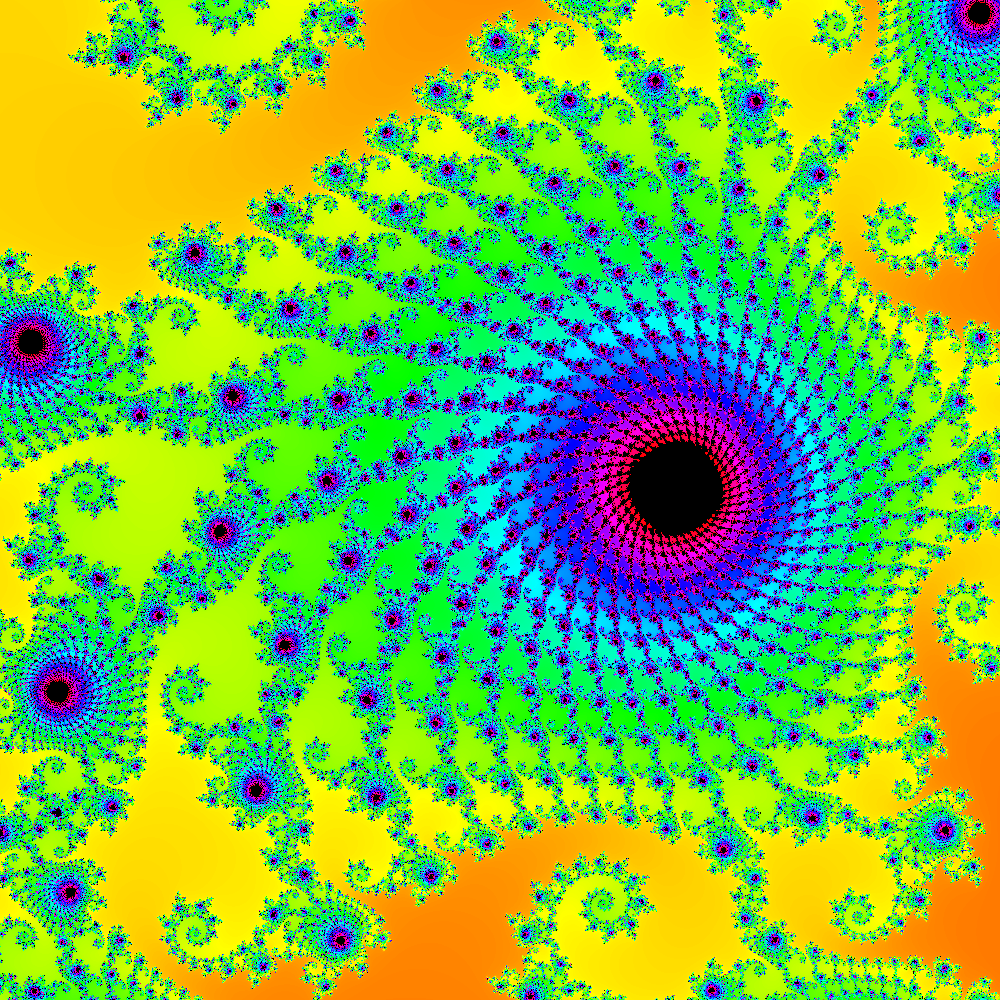
\includegraphics[width = \linewidth]{/Users/Period2/Desktop/VSCode/Mandelbrot-py/Saved Renders/Micahbrot.png}
\end{minipage}\hspace{15pt}
\begin{minipage}[t]{0.45\textwidth}
    \captionof{figure}{Fantasy}
    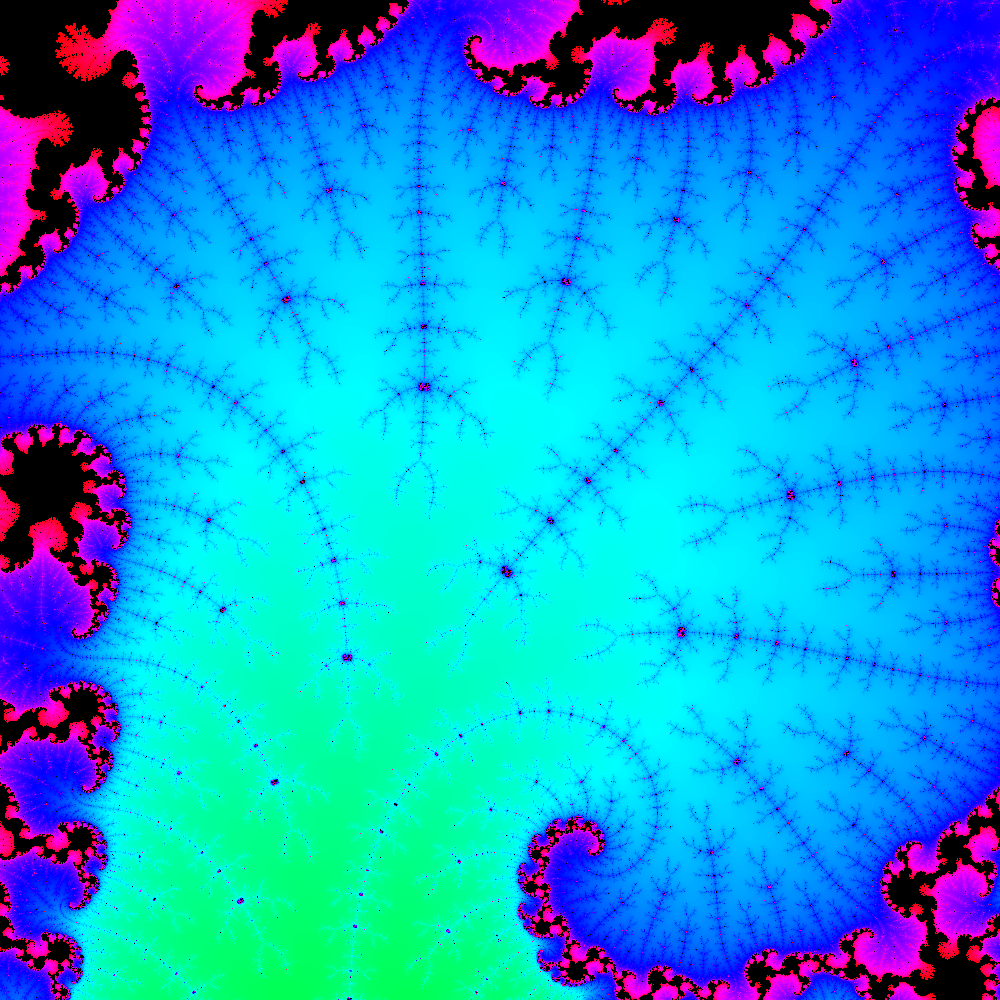
\includegraphics[width = \linewidth]{/Users/Period2/Desktop/VSCode/Mandelbrot-py/Saved Renders/Fantasy.png}
    \captionof{figure}{Hurricanes}
    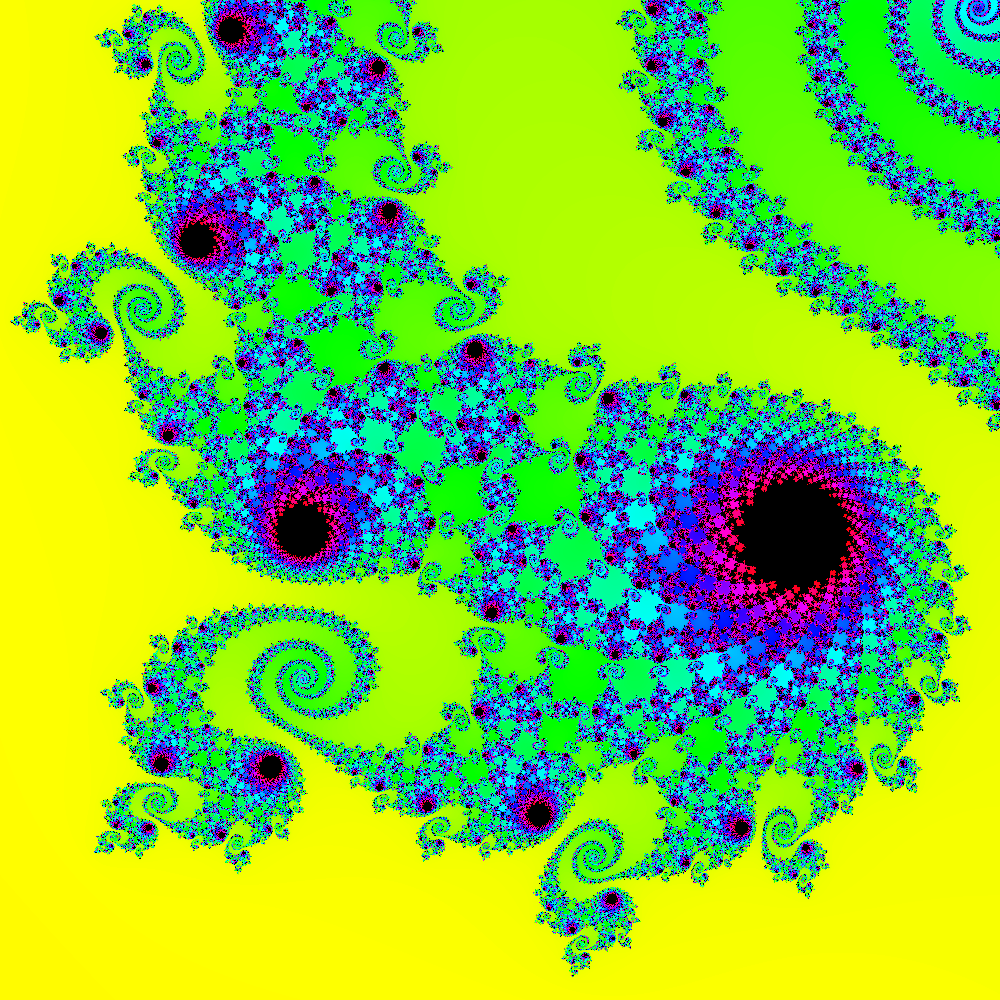
\includegraphics[width = \linewidth]{/Users/Period2/Desktop/VSCode/Mandelbrot-py/Saved Renders/Hurricanes.png}
    \captionof{figure}{Strange}
    
\includegraphics[width = \linewidth]{/Users/Period2/Desktop/VSCode/Mandelbrot-py/Saved Renders/Strange.png}
\end{minipage}
\end{document}